\def\Slide{} % Change name other than 'Slide' like 'SlideX' to make A4 paper
\def\PrintLecture{1} % Lecture On(1)/Off(0)
\def\PrintSolution{1} % Solution(Answer) On(1)/Off(0)

\def\MyClass{\R ・\RStudio のインストール}

% Include Files
\def\DirCourse{\string~/AQUOS/Default_Folder/TIU/lectures} % Manual setting
\def\MyCourse{データサイエンスコース}
\def\MySubject{R入門}
\def\MySemester{春学期}

\newcommand{\R}{\textbf{R}}
\newcommand{\RStudio}{\textbf{RStudio}}
\newcommand{\Excel}{\textbf{Excel}}
\newcommand{\cs}[1]{\textcolor{blue}{\texttt{#1}}} % Console prompt >

\input{\DirCourse/tex/macro_lualatex.tex}

\begin{document}
\ifthenelse{\Slide=1}{\date{}}{}
\maketitle
\thispagestyle{fancy}
\tableofcontents
\newpage

\section{はじめに}
\Tic{5}

統計解析は,10年ほど前までは,CやFortranなど,取扱いに専門的知識を要する
プログラミング言語を用いて行われていました.
これを,高度なプログラミング知識がなくても誰でも利用できる形にしたものが,統計解析環境\R です.
今や,データサイエンスの世界では標準のソフトウェアツールとなっています.\\[3mm]

\R を習得すれば,統計解析から業務効率化ツールの作成までオールマイティーに,
そのスキルを活用できます.\\[3mm]

手を動かして自分でやってみることが\R 習得の近道です.そのため,各スライドには,
必ず演習を載せてあります.

\section{\R}
\Tic{5}

\R とは,AT&Tベル研究所が開発した統計解析用の
プログラミング言語(S言語)
を参考にして作られたオープンソースの言語(R言語)を使用できる
統計解析環境.\\[5mm]

\begin{minipage}{0.45\textwidth}
  \begin{figure}[H]%[H] of float package is required for minipage
  \centering
  
\includegraphics[width=0.3\textwidth]{logo-r}
  \label{fig:logo-r}
  \caption{The R environment}
  \end{figure}
\end{minipage}
\hspace{3mm}
\begin{minipage}{0.45\textwidth}
  \begin{figure}[H]
  \centering
  \includegraphics[width=0.3\textwidth]{r-open.pdf}
  \label{fig:r-open}
  \caption{Microsoft R Open}
  \end{figure}
\end{minipage}

\R により,現代統計学をほぼ網羅する広範な統計解析や
出版物品質のグラフ描画が容易となる.\\[3mm]

Microsoft社により開発・保守されている高速版の\R も存在する.

\section{\R パッケージ}

\R だけでも基本的な統計解析は可能だが,
ユーザーの利用目的に応じて開発された\R パッケージと呼ばれる
統計解析ライブラリをインストールすることで機能を拡張できる.\\[3mm]

\R パッケージは,C/C++,Fortran,R言語で記述されており,
当初は,欧米大学の統計学科の教員らが中心となり
開発・保守を行っていたが,
近年は民間を含む様々な分野で広く開発が進められている.
すでに,1,000を超える\R パッケージがインターネット上で公開されている.

\section{CRAN}

CRAN(包括的R保存庫網)とは,\R の本体やパッケージ,
マニュアル類が無償公開されているウェブサイト.
ユーザーは,最寄りのミラーサイトからソフトウェアをダウンロードする.
%\R 関連のソフトウェアをダウンロードする際には,
%次の国内のサイトを利用する.

%$\rightarrow$ 統計数理研究所(\url{https://cran.ism.ac.jp})

\begin{figure}[H]
  \centering
  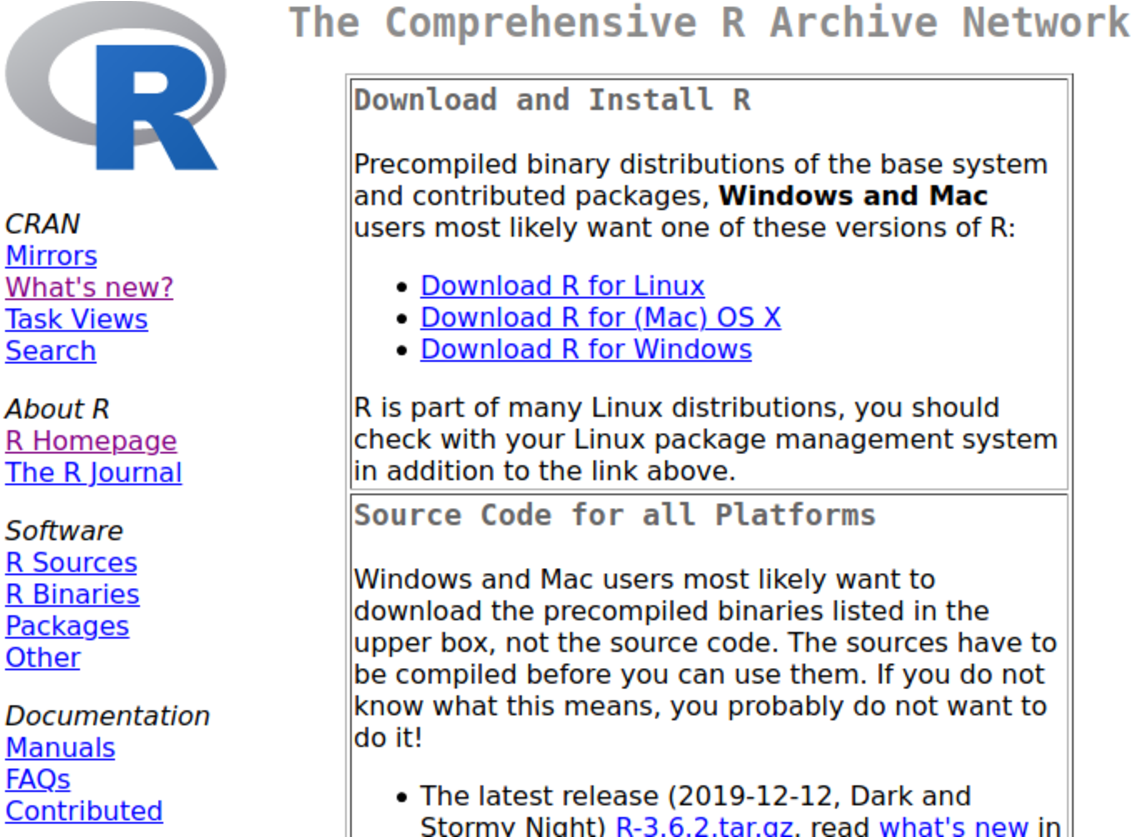
\includegraphics[width=0.6\textwidth]{cran}
  \label{fig:cran}
\end{figure}

\section{RjpWiki}

日本語での\R の情報源としては,次のウェブサイトが有名\\
多くの有用な情報が掲載されており,質問もできる.\\[5mm]
$\rightarrow$ RjpWiki(\url{http://www.okadajp.org/RWiki})

\begin{figure}[H]
  \centering
  \includegraphics[width=0.9\textwidth]{rjpwiki}
  \label{fig:rjpwiki}
\end{figure}

\section{\RStudio}

\RStudio とは,\R 用の統合開発環境(IDE)で,
ソースコードの編集,実行,ヘルプの表示,パッケージの作成など,
プログラミングに必要な様々な便利な機能を持つソフトウェア\\[3mm]
%
\begin{minipage}{0.45\textwidth}
  \begin{figure}[H]
    \centering
    
\includegraphics[width=0.8\textwidth]{logo-rstudio}
    \label{fig:logo-rstudio}
  \end{figure}
\end{minipage}
\hspace{3mm}
\begin{minipage}{0.45\textwidth}
  \begin{figure}[H]
    \centering
    \includegraphics[width=0.9\textwidth]{rstudio}
    \label{fig:rstudio}
  \end{figure}
\end{minipage}\\[3mm]

オープンソース版の\RStudio を次のサイトからダウンロードできる.
$\rightarrow$ rstudio.com(\url{https://rstudio.com})

\section{\R ・\RStudio のインストール}

\foreach \x in {1,2,...,23}
{
  \begin{figure}[H]
    \centering
    %\includegraphics[width=\textwidth,trim=2mm 2mm 2mm 2mm,clip]
    \includegraphics[width=\textwidth]
    {r_install/pages/r_install_\x.pdf}
    \label{fig:r_install_\x}
  \end{figure}
}

\end{document}
